\documentclass[tikz]{standalone}
\usepackage{tikz}
\usepackage{helvet}
\renewcommand{\familydefault}{\sfdefault}


\definecolor{pizzared}{RGB}{238, 82, 48}
\usetikzlibrary{shapes,arrows}
\tikzstyle{block} = [rectangle, draw, fill=pizzared,  text=white,
    text width=7em, text centered, rounded corners, minimum height=6em,
    font=\bfseries]
\tikzstyle{line} = [draw, -latex']

\begin{document}
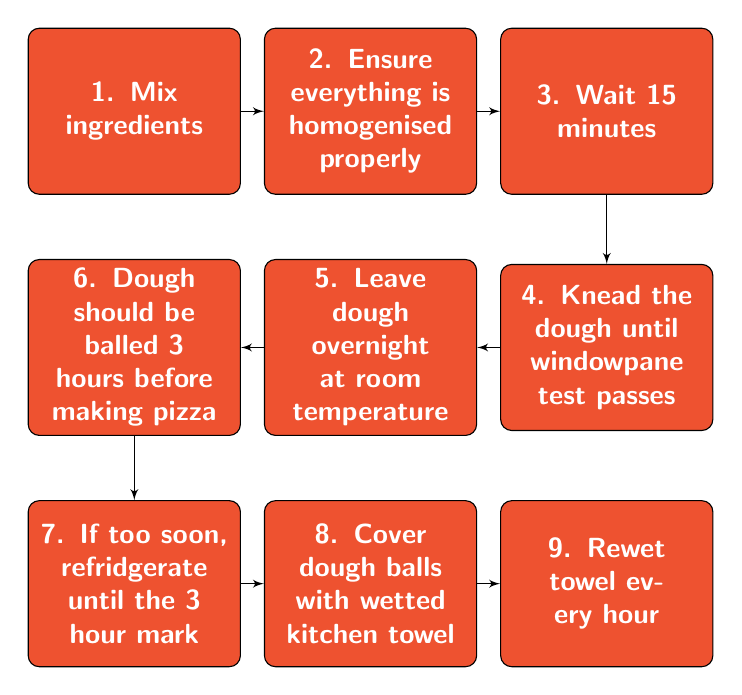
\begin{tikzpicture}[node distance = 3cm, auto]
  \node [block] (mix) {1. Mix ingredients};
  \node [block, right of=mix] (homogenise) {2. Ensure everything is homogenised properly};
  \path [line] (mix) -- (homogenise);
  \node [block, right of=homogenise] (wait) {3. Wait 15 minutes};
  \path [line] (homogenise) -- (wait);
  \node [block, below of=wait] (knead) {4. Knead the dough until windowpane test passes};
  \path [line] (wait) -- (knead);
  \node [block, left of=knead] (overnight) {5. Leave dough overnight at room temperature};
  \path [line] (knead) -- (overnight);
  \node [block, left of=overnight] (ball) {6. Dough should be balled 3 hours before making pizza};
  \path [line] (overnight) -- (ball);
  \node [block, below of=ball] (fridge) {7. If too soon, refridgerate until the 3 hour mark};
  \path [line] (ball) -- (fridge);
  \node [block, right of=fridge] (kitchen_towel) {8. Cover dough balls with wetted kitchen towel};
  \path [line] (fridge) -- (kitchen_towel);
  \node [block, right of=kitchen_towel] (rewet_towel) {9. Rewet towel every hour};
  \path [line] (kitchen_towel) -- (rewet_towel);
\end{tikzpicture}
\end{document}
